%\VignetteIndexEntry{Mulcom Manual}
%\VignetteKeywords{Expression Analysis}
%\VignetteDepends{Mulcom}
%\VignettePackage{Mulcom}
\documentclass[a4paper]{article}

\usepackage{amsmath,amssymb,pstricks}
\usepackage{graphicx}
\usepackage{Sweave}
%\setlength{\parindent}{0cm} \setlength{\parskip}{12pt}
%\renewcommand{\baselinestretch}{1.2}

\begin{document}

\title{\texttt{MulCom}: a \texttt{Mul}tiple \texttt{Com}parison statistical test for microarray 
data in Bioconductor.}

\author{Claudio Isella, Tommaso Renzulli, Davide Cor\`a and Enzo Medico}

\maketitle

\vspace{12pt}

\begin{abstract}
Many microarray experiments compare a common control group
with several "test" groups, like in the case , for example of a \emph{time-course} experiments 
where time zero serves as a common reference point. The \texttt{MulCom} 
package described here implements the Dunnett's \emph{t}-test, which has been 
specifically developed to handle multiple comparisons against a common 
reference, in a version tailored for genomic data analysis that we named 
\texttt{MulCom} (\texttt{Mul}tiple \texttt{Com}parisons) test. 
The implementation includes two test parameters, namely the \emph{t} value and 
an optional minimal fold-change value, \emph{m}, with automated, 
permutation-based estimation of False Discovery Rate (FDR) for parameter 
combinations of choice.
 
The package permits automated optimization of the test parameters to obtain the 
maximum number of significant genes at a given FDR value. In this vignette we 
present the rationale, implementation and usage of the \texttt{MulCom} package, 
plus a practical application on a \emph{time-course} microarray experiment.

\end{abstract}
\newpage
\tableofcontents
\newpage
\section{Introduction}
Together with the technical advancing of the -omics platforms and in particular 
of microarray analysis of gene expression, the bioinformatics community has 
developed several statistical tools to handle data and discriminate between truly 
differential gene regulation and systematic/random measurement errors deriving 
from the highly parallel -but poorly replicated- microarray data. Indeed, statistical 
analysis severely suffers from the limited number of replicates usually performed in 
these experiments. Typical analysis algorithms use \emph{t}-test or similars to identify 
gene lists discriminating two experimental subgroups. However, several gene 
expression experiments encompass multiple experimental points to be compared 
with a reference point. This is the case, for example, of a \emph{time-course}, or other experimental designs involving,  
multiple different treatments versus a control condition. The analysis 
is then aimed at assessing, for each gene, which experimental group means are 
significantly different from the control group mean. 

In principle, it is possible to run a \emph{t}-test-based method for each comparison. 
However, when applied to this type of data, \emph{t}-test-based methods 
have several problems: (i) they do not correct the result of each comparison for the 
total number of comparisons made; (ii) information about experimental variability 
(the standard error) is extracted only from the a limited number of samples (the two groups actually compared) and 
the possibility of very low standard error occurring by chance (and therefore of 
false positives) are very high, (iii) the estimation of the standard error 
could be overextimated, leading to a high rate of false negatives. Alternatively, one could use a procedure 
such as the \emph{Tukey}'s "Honestly Significantly Different" (HSD) test, 
designed to compare each mean with each other mean. The problem with using the 
\emph{Tukey}'s HSD is that, like any other method designed for systematic pairwise comparison of all means,
 it over corrects for the number of comparisons made, when 
the only comparisons of interest are those with the common reference. 

To tackle these issues and enable optimal analysis of multiple comparisons versus 
a reference group we designed the \texttt{MulCom} test and implemented an R-Bioconductor \cite{Gentleman} package 
which implements on the basis of a modified Dunnett's \emph{t}-test, adapted to microarray data analysis. 
The test includes an optional tunable fold-change threshold 
(\emph{m}) and Montecarlo simulation to assess FDR. 
We also implemented a streamlined procedure for automated optimization of test 
parameters, to maximize the number of significant genes at a given FDR.

The package is loaded with the command

\begin{Schunk}
\begin{Sinput}
> library(Mulcom)
\end{Sinput}
\end{Schunk}

\newpage
\section{The \texttt{MulCom} Test}

The Dunnett's \emph{t}-test is a procedure designed to compare 
different experimental conditions with a common control condition.

The procedure for comparing each experimental mean with the control mean is called 
"Dunnett's test". 


Dunnett's test controls 
the Experiment-wise Error Rate and is more powerful than tests designed to compare 
each mean with each other mean. The test is conducted by computing a modified 
\emph{t}-test between each experimental group and the control group. 
The Dunnett's \emph{t}-test formula is:
\[
t = {|M_i - M_c| \over \sqrt{2 * MSE \over n_h}}
\]

Where $M_i$ is the mean of the $i^{th}$ experimental group, $M_c$ is the mean of the control group, $MSE$
is the mean square error as computed from the analysis of variance, and \emph{$n_h$} is
the harmonic mean of the sample sizes of the experimental group and the control
group.

We integrated the Dunnett's formula a tunable \emph{m} parameter to set
a minimum threshold for differential expression, thereby obtaining what we called the \texttt{MulCom} test: 
\[
t = {|M_i - M_c| -m \over \sqrt{2 * MSE \over n_h}}
\]
where the \emph{m} parameter is subtracted from the numerator of the test.

To define the \emph{t} value threshold for significance, instead of the alpha-based 
Dunnett's tables, the FDR of the test is estimated by extensive 
sample permutations. The same approach can be used to optimally tune the \emph{m} 
parameter, which we found to substantially improve the number of significant 
genes at a given FDR.

It should be anyway notices that the \texttt{MulCom} test can be converted into the classical Dunnett's \emph{t}-test, by simply setting
\emph{m} to zero.
 
\section{Practical Example}

In this vignette th \texttt{MulCom} test is applied to  
benchmark dataset provided together with this vignette. It is a 
\emph{time-course} experiment in which MDA-MB-435 cells have been stimulated 
with Hepatocyte Growth Factor (HGF) for 0, 1, 6 and 24 hours. We also added an 
experimental point in which MDA-MB-435 cells are transduced with integrin B4 
(ITGB4) as a control (detection of significantly differential ITGB4 expression 
is expected). The experiment has been performed on Affymetrix (HGU133A) and 
Illumina (RS-8 Human Beadchip) arrays, to assess statistical test 
reproducibility on two independent platforms. In the "benchVign"
file we included the Affymetrix, "Affy", data and the cross-annotation table, "AffyIlmn". 
Data was filtered for expression calls.
%Both Affymetrix and Illumina datasets have been filtered, respectively for 
%"Presence" and "Detection Values". The criterion for maintaining a probe/probeset 
%was that at least two samples were called "Present" (Affy) or that 95\% of the samples had a "Detection Value"
%of 0.99 (Illumina). Additionally, probesets/probes lacking any annotation
%were also removed from the datasets. 

\begin{Schunk}
\begin{Sinput}
> data("benchVign")
\end{Sinput}
\end{Schunk}

\subsection{\texttt{MulCom} Analysis}
The \texttt{MulCom} implementation requires as starting imput files 
an \texttt{ExpressionSet} and a class vector corresponding 
to groups in the analysis. In this example the class vector is Affy\$Groups: 
\begin{Schunk}
\begin{Sinput}
> Affy$Groups
\end{Sinput}
\begin{Soutput}
 [1] "3" "0" "1" "2" "3" "0" "1" "2" "4" "4"
\end{Soutput}
\end{Schunk}
\texttt{MulCom} can be applied with the following procedure:
\begin{Schunk}
\begin{Sinput}
> mulcomScore <- mulScores(Affy, Affy$Groups)
\end{Sinput}
\end{Schunk}
Where \emph{mulScores} calculates the numerator and the denominator of the test without 
the parameters \emph{m} and \emph{t}. 

On this output, \emph{mulCalc} calculates the number of significant genes 
derived from the analysis in all the comparisons, with specific \emph{m} 
and \emph{t} (m = 0.3, t = 1.7) ("sg"):

\begin{Schunk}
\begin{Sinput}
> sg <- mulCalc(mulcomScore, m = 0.3, t = 3)
> sg
\end{Sinput}
\begin{Soutput}
[1] 181 220  10  35
\end{Soutput}
\end{Schunk}
\subsection{Montecarlo simulation for \texttt{MulCom} Test}
To validate the performance of the test with the chosen parameters, the package implements the function
\emph{mulPerm} to perform a Montecarlo analysis of the data, which reiterates \emph{mulScores} on permutated
samples. The function requires the \texttt{ExpressionSet}, the number of permutations, 
\emph{np}, and \emph{seed}, to generate reproducible permutation:

\begin{Schunk}
\begin{Sinput}
> permutation <- mulPerm(Affy, Affy$Groups, np = 100, seed = 7)
\end{Sinput}
\end{Schunk}

On the basis of the permutations, \emph{mulFSG} can be used to estimate the median number
of genes called in the Montecarlo model ("fsg") and thus estimate the FDR.

\begin{Schunk}
\begin{Sinput}
> fsg <- mulFSG(permutation, m = 0.3, t = 3)
> fsg
\end{Sinput}
\begin{Soutput}
[1] 2.5 3.0 3.0 2.0
\end{Soutput}
\begin{Sinput}
> fdr <- fsg/sg
> fdr
\end{Sinput}
\begin{Soutput}
[1] 0.01381215 0.01363636 0.30000000 0.05714286
\end{Soutput}
\end{Schunk}

This result revealed that with \emph{m} = 0.3 and \emph{t} = 3 applied to the whole dataset, two out of four comparison have a FDR below 0.05. 
Indeed, every comparison requires an independent tuning of the \texttt{MulCom} test parameters.

To facilitate optimization of the test parameters, we developed a streamlined analysis strategy.
The \emph{mulOpt} function will recursively calculate the \texttt{MulCom} test across all the experiments
with specific series of \emph{m} and \emph{t} defined by the user, provided as vectors.

\begin{Schunk}
\begin{Sinput}
> optimization <- mulOpt(permutation, vm = seq(0, 0.5, 0.1), vt = seq(1, 
+     3, 0.1))
\end{Sinput}
\end{Schunk}

The function \emph{mulParOpt} is designed to identify the optimal \emph{m} and 
\emph{t} values combination leading to the maximum number of differentially 
regulated genes satisfying an user define FDR threshold. 

The function  requires the \texttt{ExpressionSet}, the output of the \emph{mulOpt}, an
index, \emph{ind} defining the comparison to optimize and a threshold, \emph{ths}, 
defining the  FDR required. In case of equal number of genes, the combination of \emph{m} and \emph{t} with 
the lower FDR will be prioritized. In case of both identical number of genes and FDR, 
the function will chose the highest \emph{t}. The function optionally will define a graphical
output to visually inspect  the performance of the test at given \emph{m} and 
\emph{t} parameters for a certain comparison. 
\begin{Schunk}
\begin{Sinput}
> h1Opt <- mulParOpt(permutation, optimization, ind = 1, th = 0.05)
\end{Sinput}
\begin{Soutput}
[1] 946
\end{Soutput}
\end{Schunk}
In this case the optimization with FDR = 0.05 yielded \emph{t} = 1.7 and \emph{m} = 0.3
\begin{Schunk}
\begin{Sinput}
> h1Opt
\end{Sinput}
\begin{Soutput}
  t   m 
1.5 0.3 
\end{Soutput}
\end{Schunk}
\begin{figure}[!ht]
\begin{center}
\begin{Schunk}
\begin{Soutput}
[1] 946
\end{Soutput}
\end{Schunk}
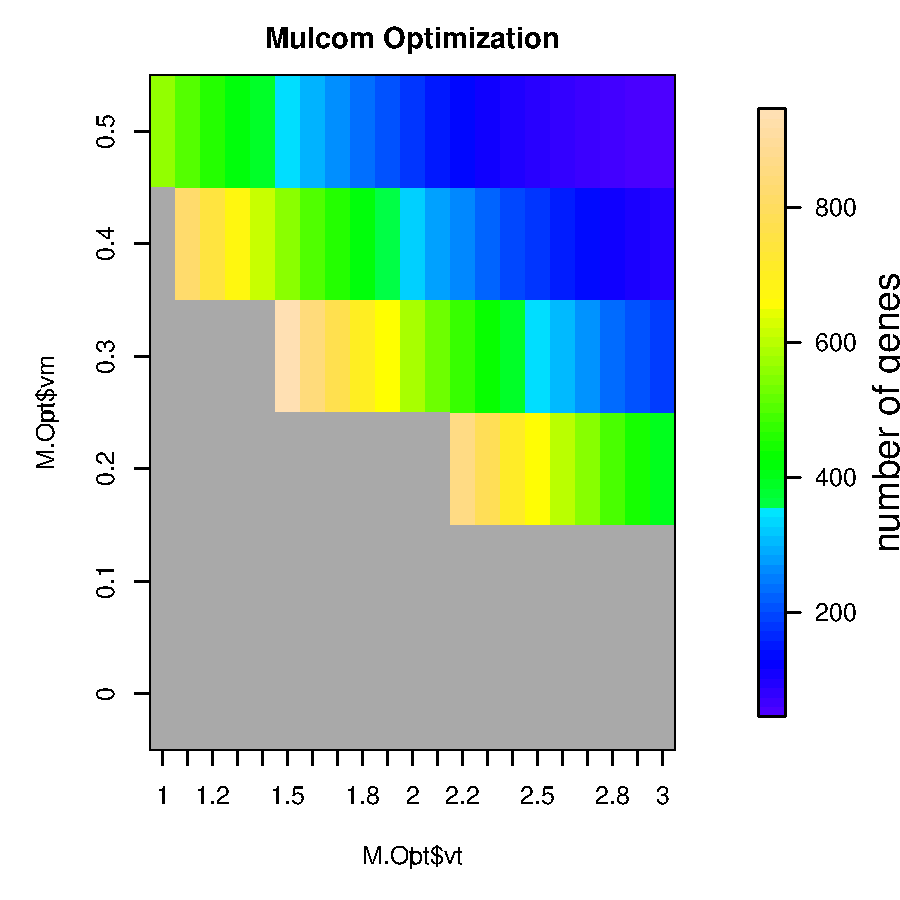
\includegraphics{MulcomVignette-ThresholdOptimization}
\end{center}
\caption{\emph{\scriptsize{plot for \texttt{MulCom} Figure 1: plot for MulCom Test optimization: The plot shows the number of significant
genes for a series of combinations of m and t. The grey area represents the combinations that do not reach the FDR of choice}}}
\end{figure}
\newpage

In the example below we adopt the automated method to optimize \emph{m} and
\emph{t} with \emph{mulParOpt} and the function \emph{mulDiff} to identify differentially regulated
genes. \emph{mulDiff} requires the \texttt{ExpressionSet}, the permutation object and the \emph{m}
and \emph{t} parameters:

\begin{Schunk}
\begin{Sinput}
> h1Opt <- mulParOpt(permutation, optimization, ind = 1, th = 0.05)
\end{Sinput}
\begin{Soutput}
[1] 946
\end{Soutput}
\begin{Sinput}
> affyMulc1Probes <- mulDiff(Affy, permutation, m = h1Opt[2], t = h1Opt[1], 
+     ind = 1)
\end{Sinput}
\end{Schunk}
The analysis performed on first comparison yielded 902 differentially expressed genes,
with an FDR below 5\%.
\begin{Schunk}
\begin{Sinput}
> h6Opt <- mulParOpt(permutation, optimization, ind = 2, th = 0.05)
\end{Sinput}
\begin{Soutput}
[1] 886
\end{Soutput}
\begin{Sinput}
> affyMulc6Probes <- mulDiff(Affy, permutation, h6Opt[2], h6Opt[1], 
+     2)
\end{Sinput}
\end{Schunk}
\begin{Schunk}
\begin{Sinput}
> h24Opt <- mulParOpt(permutation, optimization, ind = 3, th = 0.1)
\end{Sinput}
\begin{Soutput}
[1] 4
\end{Soutput}
\begin{Sinput}
> affyMulc24Probes <- mulDiff(Affy, permutation, h24Opt[2], h24Opt[1], 
+     3)
\end{Sinput}
\end{Schunk}
\begin{Schunk}
\begin{Sinput}
> b4Opt <- mulParOpt(permutation, optimization, ind = 4, th = 0.05)
\end{Sinput}
\begin{Soutput}
[1] 28
\end{Soutput}
\begin{Sinput}
> affyMulcB4Probes <- mulDiff(Affy, permutation, b4Opt[2], b4Opt[1], 
+     4)
\end{Sinput}
\end{Schunk}
\begin{Schunk}
\begin{Sinput}
> mulcomGeneList <- unique(c(affyMulc1Probes, affyMulc6Probes, 
+     affyMulcB4Probes))
\end{Sinput}
\end{Schunk}
The analysis yielded to 1555 significant genes; we performed the same analysis on Illumina dataset: with 763 significant genes 
\section{Discussion}
The \texttt{MulCom} package provides a simple and powerful tool for the
identification of differentially expressed genes between a control and
several experimental conditions. This algorithm is better
suited for multiple comparisons than \emph{t}-tests performing
single pairwise comparisons, as it estimates the
within-group variability across all experimental groups.
